\documentclass[a4paper]{jacow}
\usepackage{mathtools}
\usepackage{amsmath}
\usepackage{xfrac}
\usepackage{xparse}
\usepackage{subcaption}
\usepackage{graphicx}
\usepackage{url}
\usepackage{paralist}
\usepackage{multirow}
\usepackage{siunitx}
\usepackage{threeparttable}

\let\oldvec\vec
\renewcommand{\vec}{\boldsymbol}
\DeclareDocumentCommand{\bkt}{sm}{\IfBooleanTF{#1}{\left[ #2 \right]}{\left(#2\right)}}
\DeclareDocumentCommand{\ddt}{m}{\frac{\mathrm{d} {#1}}{\mathrm{d} t}}
\DeclareDocumentCommand{\pddx}{mO{t}O{}}{\frac{\partial^{#3} {#1}}{\partial {#2}^{#3}}}
\newcommand{\w}{\omega}
\newcommand{\W}{\Omega}
\newcommand{\avg}[1]{\langle {#1} \rangle}
\newcommand{\nbar}{\bar n}


\begin{document}
\title{Spin Motion Perturbation Effect on the EDM Statistic in the Frequency Domain Method}
\author{A. E. Aksentyev\textsuperscript{1,2,3}\thanks{alexaksentyev@gmail.com},
  Y. V. Senichev\textsuperscript{3}, \\
  \textsuperscript{1} National Research Nuclear University ``MEPhI,'' Moscow, Russia \\
  \textsuperscript{2} Institut f\"ur Kernphysik, Forschungszentrum J\"ulich, J\"ulich, Germany\\
  \textsuperscript{3} Institute for Nuclear Research of the Russian Academy of Sciences, Moscow, Russia}
\maketitle

\begin{abstract}
  The spin precession axis of a particle involved in betatron motion precesses about the invariant spin axis
  defined on the closed orbit (CO). This precession can be observed in polarization data as a rapid,
  small-amplitude oscillation on top of the major effect oscillation caused by the precession of spin
  about the CO axis. The frequency of this latter oscillation is used in the Frequency Domain methodology
  as the EDM observable. It is estimated by fitting polarimetry data by a sine function; the rapid
  oscillations, therefore, constitute a model specification error.
  This model error will introduce a bias into the frequency estimate. In the present work we investigate
  how this bias changes depending on the beam revolution direction, its stability over time, and
  the EDM estimate error introduced by it.
\end{abstract}

\section{Frequency Domain methodology}
Frequency Domain (FD)~\cite{Senichev:FDM} is a Storage Ring method of search for the
Electric Dipole Moment (EDM) of a fundamental particle.~\cite{BNL:SREDM}
It belongs to the Frozen Spin~\cite{BNL:Deuteron2008} category
of such methods, i.e., the Magnetic Dipole Moment (MDM) component of spin precession is minimized. However,
the original Frozen Spin method proposed in~\cite{BNL:Deuteron2008} is a Space Domain
method~\cite[p.~4]{Talman:ElectricRings}: inferences about the EDM are drawn from the change of orientation
of the polarization vector, as measured by the angle between its initial and final orientations. This approach
has the following problems:
\begin{inparaenum}[\itshape a\upshape)]
\item it puts very stringent constraints on the precision of the accelerator optical element alignment, and
\item it poses a challenging task for polarimetry.~\cite[p.~6]{Mane:SpinWheel}
\end{inparaenum}

The former is to minimize the magnitude of
the vertical plane MDM precession frequency~\cite[p.~11]{BNL:Deuteron2008}
\begin{equation}\label{eq:BNL_syst_err}
\w_{syst} \approx \frac{\mu\avg{E_v}}{\beta c\gamma^2},
\end{equation}
induced by field imperfections. The latter is due to the requirement of detecting a change of about
$5\cdot 10^{-6}$ to the cross section $\varepsilon_{LR}$ in order to get to the EDM sensitivity level
of $10^{-29}~e\cdot cm$.~\cite[p.~18]{BNL:Deuteron2008}

EDM search methods in the Frequency Domain circumvent the above problems: EDM inferences are based
on measurments of the EDM contribution to the spin precession angular velocity. The polarization vector is made to
roll about a nearly-constant, definite direction vector $\nbar$, with an angular velocity
that is high enough for the beam polarization to be easily measureable at all times. This ``Spin Wheel'' may be
externally applied~\cite{Koop:SW}, or otherwise the machine imperfection fields
may be utilized for the same purpose (wheel roll rate determined by
equation~\eqref{eq:BNL_syst_err}).~\cite{Senichev:FDM} The latter is made possible
by the fact that $\w_{syst}$ changes sign when the beam revolution direction
is reversed.~\cite[p.~11]{BNL:Deuteron2008}

The frequency of oscillation of the vertical polarization component $P_y$ is estimated
via fit of the model
\begin{equation}\label{eq:fit_model}
  f(t) = a\cdot\sin(\w\cdot t + \delta),
\end{equation}
to polarimetry data.

\section{Problem statement}
\newcommand{\ntrn}{n_{turn}}
Consider the case of a single particle beam. The solution of the T-BMT equation for the
vertical spin-vector component has the general form
\begin{equation}\label{eq:sy_growth_1}
  s_y(t) = \sqrt{\bkt{\frac{\w_y\w_z}{\w^2}}^2 + \bkt{\frac{\w_x}{\w}}^2}\cdot\sin\bkt{\w\cdot t + \delta},
\end{equation}
where $\vec\w = (\w_x, \w_y, \w_z)$ is a function of time as a result of betatron motion.

Using $\vec\w = 2\pi f_{rev}\nu_s\nbar$~\cite[p.~4]{COSY:SpinTuneMapping}, equation~\eqref{eq:sy_growth_1}
can be reformulated in terms of spin tune $\nu_s$ and invariant spin axis $\bar n$:
\begin{equation}\label{eq:main}
  s_y(n_{turn}) = \sqrt{\bkt{\nbar_y\nbar_z}^2 + \nbar_x^2}\cdot\sin\bkt{2\pi\nu_s\cdot\ntrn + \delta},
\end{equation}
where $\nbar = \nbar(\ntrn)$ and $\nu_s = \nu_s(\ntrn)$ are functions of the turn number $\ntrn$.

Sufficiently large variation of~ $\nbar$ and/or $\nu_s$ can lead to model specification systematic error.
Variation in $\nu_s$ is especialy problematic in this regard, as it directly affects the phase of the signal;
however, this problem can be solved by the introduction of sextupole fields into the system,
as described in~\cite{Aksentev:DecohIPAC19}. In this paper we will, therefore, be concerned only with the $\nbar$
variation.

\section{Simulation}
The simulation was set up as follows: a particle, offset from the design orbit in the vertical
direction by 0.3 mm, is injected multiple times into an imperfect
Frozen Spin lattice~\cite{Senichev:Lattices} utilizing sextupoles for
the reduction of spin decoherence caused by vertical plane betatron
oscillations~\cite{Aksentev:DecohIPAC19}. Lattice imperfections are simulated by rotations of the E+B spin
rotator elements. Imperfections introduced this way do not perturb the design orbit.

Each injection, the rotation angles are randomly generated from the
normal distribution $\alpha\sim N(\mu_i, 3\cdot 10^{-4})$ degrees, $i\in\{1,\dots,41\}$, where
$\mu_i$ varies in the range $[-1.5\cdot10^{-4}, +2.5\cdot10^{-4}]$ degrees. The non-zero expectation values $\mu_i$
simulate the application of a Koop Spin Wheel (SW).~\cite{Koop:SW} The magnitudes of $\mu_i$ and $\sigma_{\alpha}$
are chosen for effect detalization purposes.

Another aspect of the simulation worth noting, is that injection occurs at 270 MeV, while the FS condition
is fullfilled exactly at 270.0092 MeV. Because of that the invariant spin axis $\nbar$
points mainly in the vertical direction (deviating from it by no more than \ang{51} at higher SW roll rates);
its radial component (the one determining the oscillation amplitude of the vertical spin-vector component)
is relatively small, and all the more susceptible to variation caused by vertical plane betatron motion for that. 

Spin tracking is done in COSY Infinity~\cite{COSYINF:Website}, for $1.2\cdot10^6$ turns; each 800 turns
$\nu_s$ and $\nbar$ are computed (by means of procedure TSS~\cite[p.~41]{COSYINF:BeamPhysMan}) at
the phase space point occupied by the particle at the time, giving us the series $(\nu_s(n), \nbar(n))$.
The corresponding spin vector components $(s_x^{trk}(n), s_y^{trk}(n), s_z^{trk}(n))$,
computed by the tracker (procedure
TR~\cite[p.~41]{COSYINF:BeamPhysMan}), 
constitute the second series used in the analysis.

\section{Analysis}
Using the first series data, we generated the expected $s_y^{gen}(t)$ ``generator'' series according to
equation~\eqref{eq:main}, as well as the ``ideal'' series $s_y^{idl}$, in which
we assumed constant values of $\nu_s = \avg{\nu_s(t)}$ and $\nbar
=\avg{\nbar(t)}$. 

Our hypothesis is that the particle's betatron
motion should introduce a mismatch between the sinusoidal
model~\eqref{eq:fit_model} and tracker data, by varying the direction
of the spin precession axis $\nbar$, and hence the amplitude of the
fitted signal. The ``ideal'' series serves as the baseline of our
analysis, as it's a perfect match to the model; the ``generator''
series incorporates $\nbar$ variation, still remaining within the confines of
the model. The ``tracker'' series is the closest approximation to
real measurement data.

To compare these series with one another, we
\begin{inparaenum}[\itshape a\upshape)]
\item computed and analyzed residuals
  $\epsilon_1(t) = s_y^{gen}(t) - s_y^{idl}(t)$, and
  $\epsilon_2(t) = s_y^{trk}(t) - s_y^{idl}(t)$;
\item fitted model~\eqref{eq:fit_model} to the three time series and
  compared its goodness-of-fit;
\item computed the standard deviations of $\nbar$ components at each
  spin wheel strength.
\end{inparaenum}

\begin{figure}[h]
  \centering
    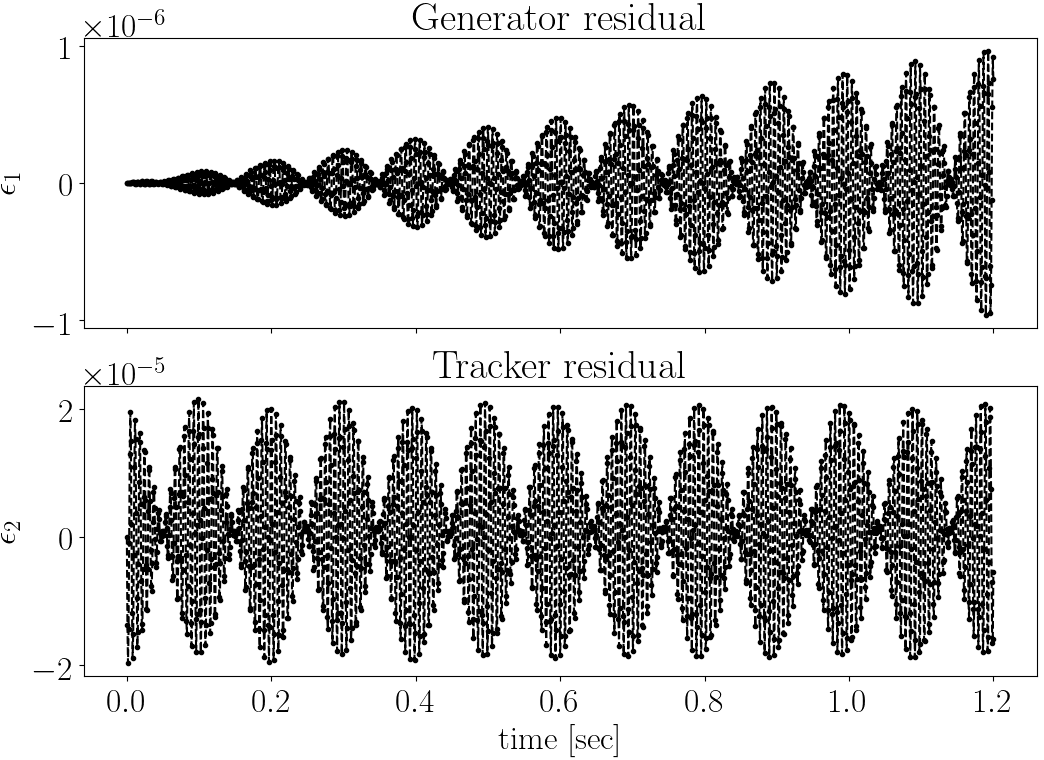
\includegraphics[width=\linewidth]{../img/IPAC19/residual_vs_time(both)}
  \caption{Time series' comparator residual as a function of time.
    Top panel: residual $\epsilon_1$; bottom panel: residual $\epsilon_2$\label{fig:residuals}}
\end{figure}

\begin{figure}[h]
  \centering
  \begin{subfigure}{\linewidth}
    \centering
    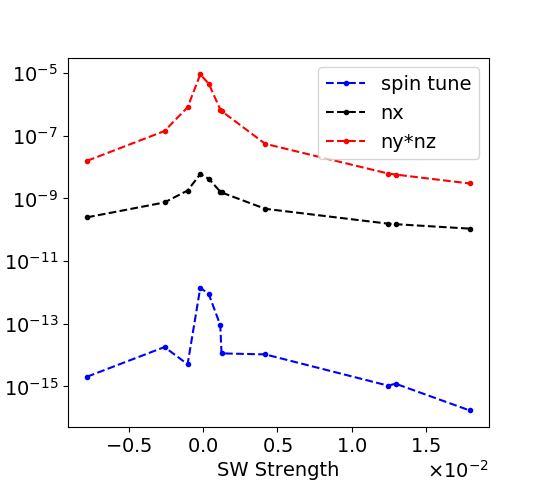
\includegraphics[width=\linewidth]{../img/IPAC19/NBAR_variation_sd_vs_SW}
    \caption{Of the $\nbar$ components\label{fig:sd:nbar}}
  \end{subfigure}
  \begin{subfigure}{\linewidth}
    \centering
    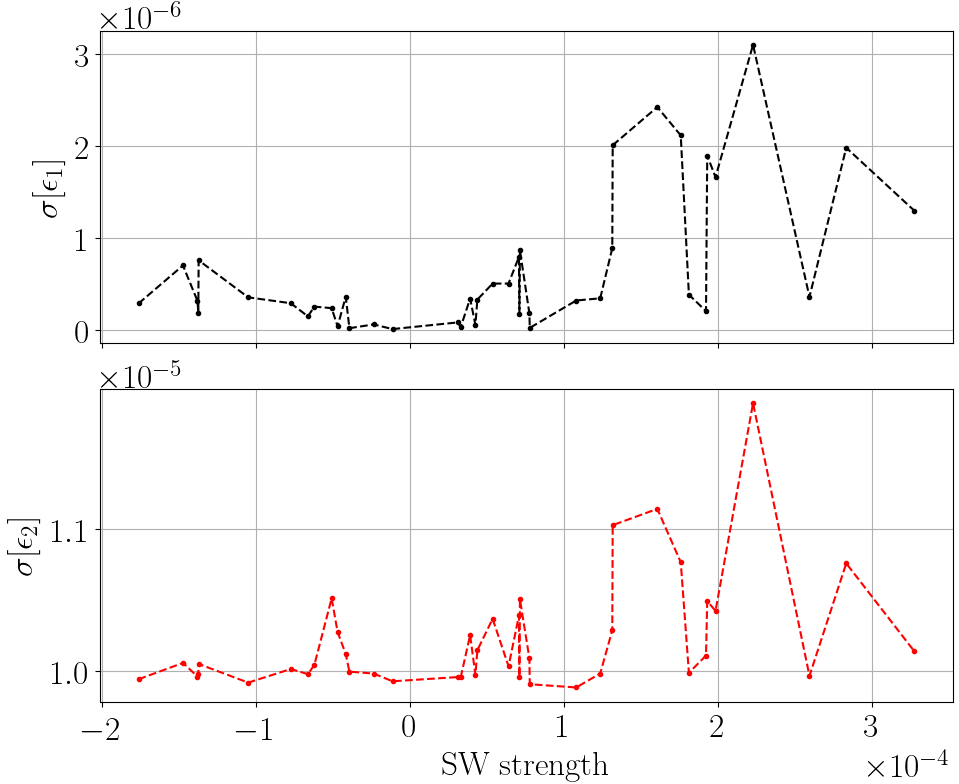
\includegraphics[width=\linewidth]{../img/IPAC19/residual_SD_vs_SW(both)}
    \caption{Of the comparator residuals.
      Top panel: residual $\epsilon_1$; bottom panel: residual $\epsilon_2$\label{fig:sd:res}}
  \end{subfigure}
  \caption{Standard deviations versus relative Spin Wheel strength ($\avg{\alpha}$)\label{fig:sd}}
\end{figure}

\begin{table}[h]
  \caption{Model parameter estimates (slowest SW roll)\label{tbl:param_estimates}}
  \begin{threeparttable}
    \begin{tabular}{r|rllr}
      \toprule
      Data & Par. & Value & St.Error & AIC\tnote{1} \\
      \midrule
      \multirow{3}{*}{$s_y^{idl}$}
      & $\hat f$ & 4.220359687911 & $6.9\cdot 10^{-11}$ & \multirow{3}{*}{-62093} \\
      & $\hat a$ & 0.12514597851 & $4\cdot 10^{-11}$ & \\
      & $\hat\delta$ & $-1.50\cdot 10^{-8}$ & $4\cdot 10^{-10}$ &\\
      \hline
      \multirow{3}{*}{$s_y^{gen}$}
      & $\hat f$ & 4.2203596911 & $1.9\cdot 10^{-9}$ & \multirow{3}{*}{-52142} \\
      & $\hat a$ & 0.125145979 & $1\cdot 10^{-9}$ & \\
      & $\hat\delta$ & $-1.6\cdot 10^{-8}$ & $1.2\cdot 10^{-8}$ &\\
      \hline
      \multirow{3}{*}{$s_y^{trk}$}
      & $\hat f$ & 4.2203603 & $1.3\cdot 10^{-6}$ & \multirow{3}{*}{-34567} \\
      & $\hat a$ & 0.12514597 & $3.7\cdot 10^{-7}$ & \\
      & $\hat\delta$ & $-4\cdot 10^{-6}$ & $6\cdot 10^{-6}$ &\\
      \bottomrule
    \end{tabular}
    \begin{tablenotes}
      \item[1] Akaike Information Criterion.
    \end{tablenotes}
  \end{threeparttable}
\end{table}

What we observe in Figure~\ref{fig:residuals} is that the ``generator'' series is nearly identical
to the ``ideal'' series (even if its frequency is slightly different), with $\epsilon_1 \le 1\cdot10^{-6}$
during run time,
while the ``tracker'' series deviates from it at the level
$\epsilon_2 \le 2\cdot 10^{-5}$. This discrepancy between $\epsilon_1$ and $\epsilon_2$ is observed
systematically across all spin wheel strengths (cf. Figure~\ref{fig:sd:res}), and has no explanation as of yet.

In Figure~\ref{fig:sd:res} we see that the standard deviations of both residuals exhibit the same
relative SW strength (as measured by $\avg{\alpha}$) dependence pattern as
the standard deviation of $\nu_s$ (Figure~\ref{fig:sd:nbar}, bottom panel), but not as that of
the $\nbar$ components. This is an indication that frequency variation is a much more significant factor
in the mismatch between model~\eqref{eq:fit_model} and tracker data, than is the presumed amplitude variation
due to the change of orientation of $\nbar$.

Table~\ref{tbl:param_estimates} characterizes the fit model's goodness-of-fit with respect to the time series,
in the case of the slowest-rolling Koop Wheel.
One observes that the differences between the parameter estimates of all three series are not
statistically significant. Even though variation of the spin precession angular velocity vector worsened
the fit quality of the model, it didn't introduce any statistically-significant bias
into the estimates.

\section{Conclusions}
The question of the influence of betatron motion on the EDM statistic in the FD method should be considered
in view of three circumstances:
\begin{enumerate}
\item The signal amplitude oscillations (as estimated by $\epsilon_2$) are small.
  They occur at the $10^{-4}$ level (when $\alpha\sim N(0, 3\cdot 10^{-2})$ degrees), whereas
  the expected polarization measurement error is on the order of percents.
  This means the superposition of this systematic error with the random measurement error
  will exhibit no statistically-significant systematicity.
\item The correllation coefficient between the amplitude and frequency estimates is not significant. The amplitude
  oscillations affect the $\hat a$-estimate foremost; their effect on the $\hat\w$-estimate is secondary, and is
  described by the correlation coefficient. Since it is less than 10\%, even if the oscillations happen to be
  strong enough to affect the amplitude estimate, their effect on the frequency estimate will be reduced by
  at least a factor of 10.
\item This systematic effect is controllable. And this point is the major advantage of the FD methodology.
  By applying an external Spin Wheel, the $\nbar$ oscillations can be continuously minimized
  as much as necessary, without changing the experiment pattern.
\end{enumerate}

\begin{thebibliography}{9}

\bibitem{Senichev:FDM}
  Y. Senichev, A. Aksentev, A. Ivanov, E. Valetov, ``Frequency domain method of the search for
  the deuteron electric dipole moment in a storage ring with imperfections,'' arxiv:1711.06512 [physics.acc-ph]
  \url{https://arxiv.org/abs/1711.06512}.

\bibitem{BNL:SREDM}
  M. Bai et al., SREDM Collaboration website: \url{https://www.bnl.gov/edm/}.

\bibitem{BNL:Deuteron2008}
  D. Anastassopoulos et at., (srEDM Collaboration), ``Search for a permanent electric dipole moment of
  the deuteron nucleus at the $10^{-29}~e\cdot cm$ level,'' proposal as submitted to the BNL PAC, April 2008.

\bibitem{Talman:ElectricRings}
  R. Talman, ``Prospects for Electric Dipole Moment Measurement Using Electrostatic Accelerators,''
  Reviews of Accelerator Science and Technology, A. Chao and W. Chou, editors, Volume 10, 2018, not yet in print.

\bibitem{Mane:SpinWheel}
  S. Mane, ``A distillation of Koop's idea of the Spin Wheel,'' arXiv:1509.01167 [physics]
  \url{http://arxiv.org/abs/1509.01167}.

\bibitem{Koop:SW}
  I. Koop. ``Asymmetric energy colliding ion beams in the EDM storage ring,'' Proc. of IPAC13 (2013).
  \url{http://accelconf.web.cern.ch/accelconf/ipac2013/papers/tupwo040.pdf}.

\bibitem{COSY:SpinTuneMapping}
  A. Saleev et al., (JEDI Collaboration), ``Spin tune mapping as a novel tool to probe
  the spin dynamics in storage rings.'' Phys. Rev. Accel. Beams 20 (2017) no.7, 072801.

\bibitem{Aksentev:DecohIPAC19}
  A. Aksentev, Y. Senichev, ``Spin decoherence in the Frequency Domain Method for the search of a particle EDM,''
  presented at the 10th International Particle Accelerator Conf. (IPAC’19), Melbourne, Australia,
  May. 2019, paper 2738, this conference.

\bibitem{Senichev:Lattices}
  Y. Senichev, S. Andrianov, S. Chekmenev, M. Berz, E.Valetov. ``Investigation of Lattice for Deuteron EDM Ring,''
  Proc. of ICAP15 (2015). \url{http://accelconf.web.cern.ch/AccelConf/ICAP2015/papers/modbc4.pdf}.

\bibitem{COSYINF:Website}
  M. Berz, K. Makino, COSY Infinity website: \url{cosyinfinity.org}.

\bibitem{COSYINF:BeamPhysMan}
  M. Berz, K. Makino. COSY INFINITY 10.0 Beam Physics Manual.

\end{thebibliography} 
\end{document}
